\subsection{インヒビット回路}
\label{subsec;inhibit}

射場作業から衛星分離までの期間における意図しない電波放射を防ぐ,あるいは放出ポッド搭載から放出までの太陽電池からの電源供給を遮断する等の目的のために,文献 \cite{sat_safety}を参考に3インヒビット回路を本衛星に設けた.購入品の機能ではこの要求を満たせなかったため,Battery-EPS間に新たに通信・インヒビット基板(Communication \& Inhibit circuit Board, CIB)を設けた(図\ref{fig3-1cib_p},\ref{fig3-1cib}).

\begin{figure}[htbp]
	\centering
	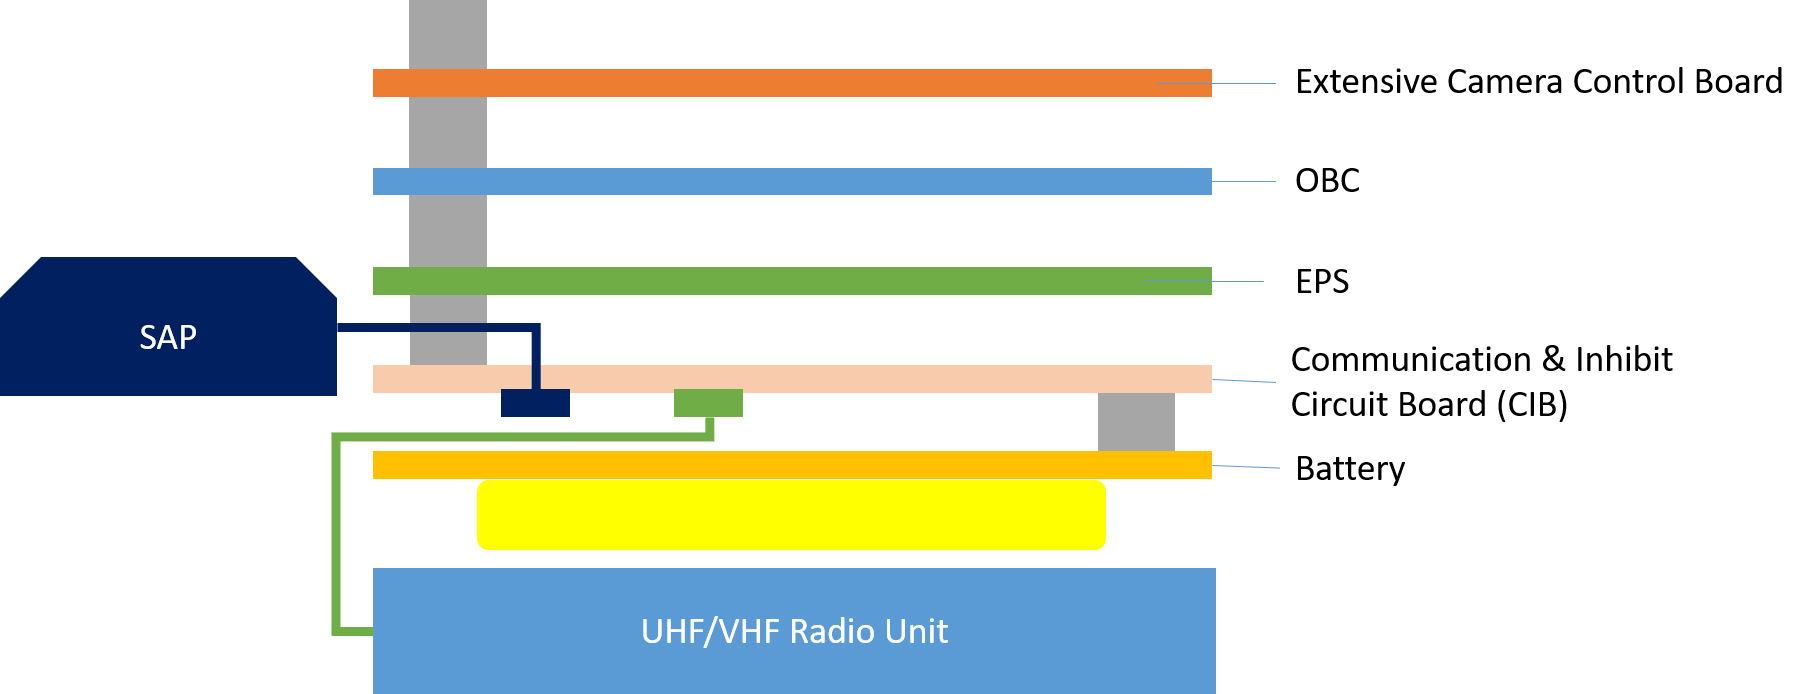
\includegraphics[width=0.7\linewidth]{./03/fig/cib_position.png}
	\caption{Overview of Satellite Bus Components}
	\label{fig3-1cib_p}
\end{figure}

\begin{figure}[htbp]
	\begin{minipage}{0.5\hsize}
		\begin{center}
			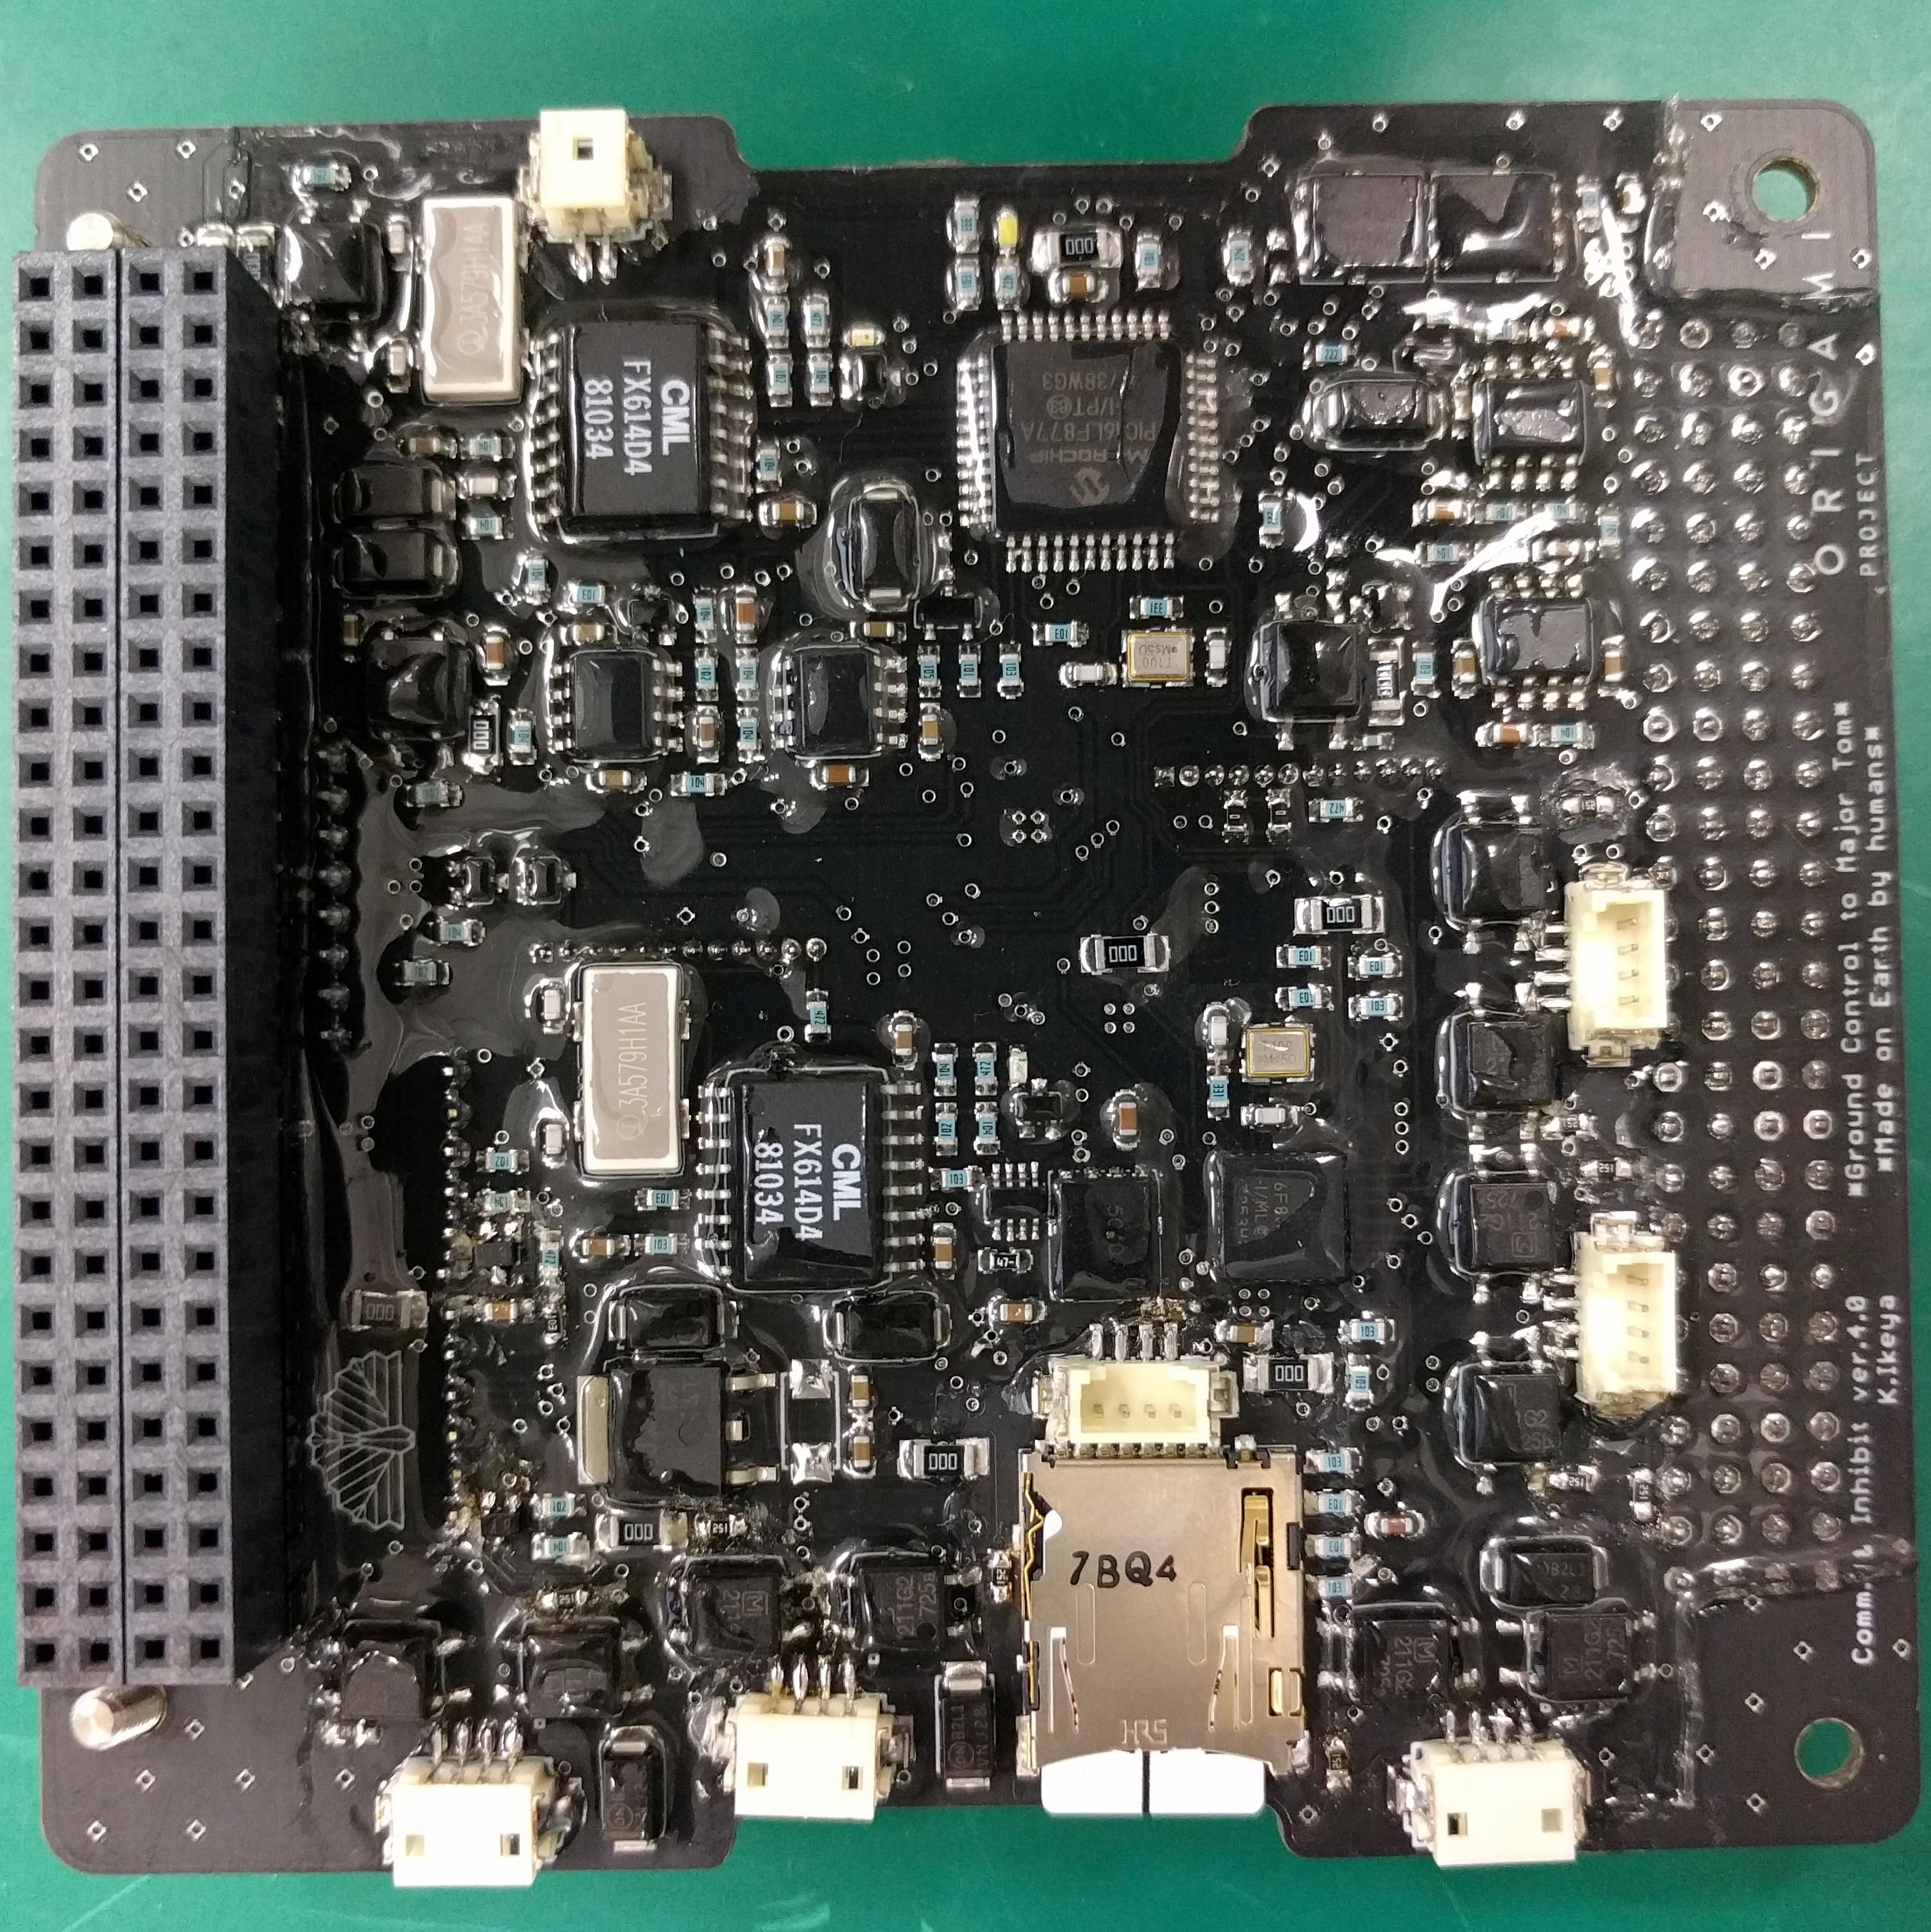
\includegraphics[width=0.7\linewidth]{./03/fig/CIB_1.jpg}
		\end{center}
	\end{minipage}
	\begin{minipage}{0.5\hsize}
		\begin{center}
			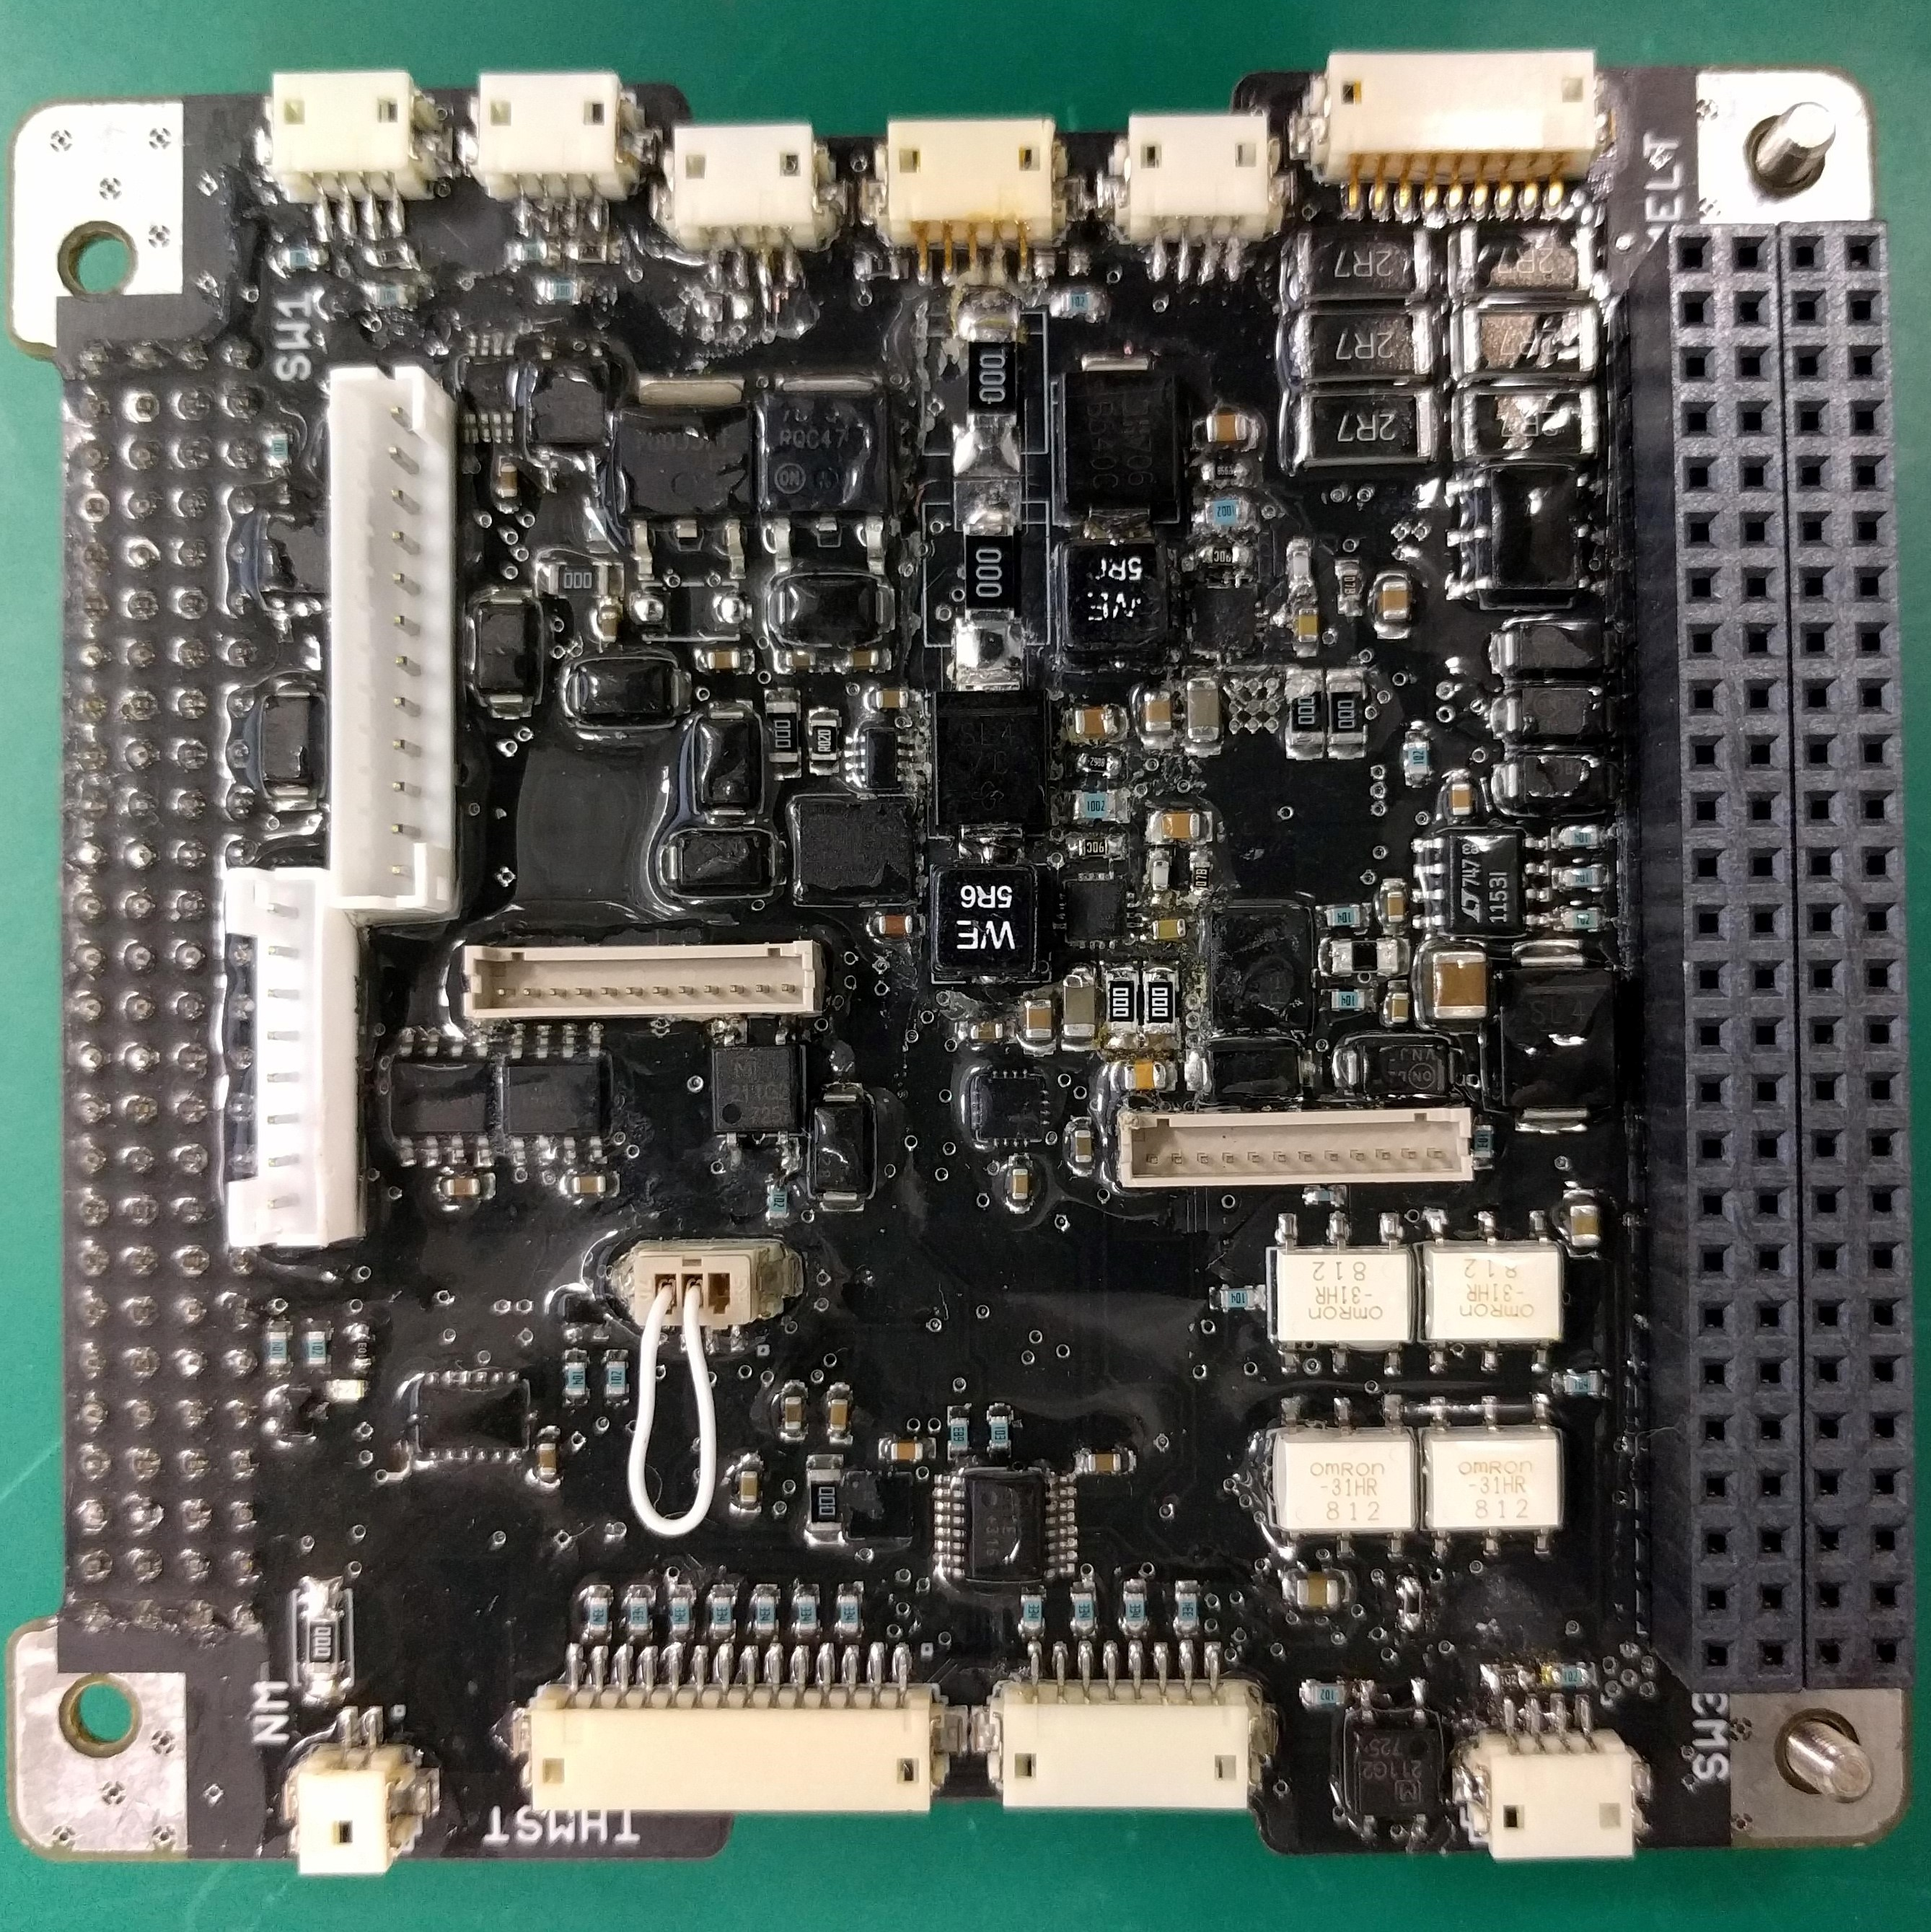
\includegraphics[width=0.7\linewidth]{./03/fig/CIB_2.jpg}
		\end{center}
	\end{minipage}\\		
	\begin{center}
		\caption{Image of CIB}
	\end{center}
	\label{fig3-1cib}
\end{figure}


インヒビット回路の回路図は図\ref{fig3_1_inhibit_d}のようになっている.購入したEPSの仕様上Battery-EPS間のみならず,SAP-EPS間も遮断し,SAPに光が当たっていてもEPSが動作しないようにした(図\ref{fig3-1_eps_bd}参照).

COLD側のMOSFETはON Semiconductor社のNTMFS5C404NをBack to Backで接続した.これは電流を双方向に流すことが目的であったが実際にはEPS側からバッテリ側にのみ流れるため,MOSFET内のドレイン・ソース間オン抵抗,および基板実装を考慮し,片方のみが好ましい.

HOT側のソリッドステートリレーはBattery-EPS間にオムロン株式会社のG3VM-31HRを,SAP-EPS間にはパナソニック株式会社AQY211G2を選定した.これは低オン抵抗であることを重要視して選定した.HOT側のインヒビットはP-chanel MOSFETとN-channel MOSFETを組み合わせても(充放電ともにできるよう設計しなければならないが)実現可能である.本衛星では回路の簡易化のためにソリッドステートリレーを選択したものの,MOSFETのほうが概して内部抵抗が小さいため基板の面積との兼ね合いではMOSFETによる遮断も検討する必要がある.


これらのIC動作の不具合は衛星にとって致命的であるため実証実績の少ないソリッドステートリレーは並列に接続し冗長系を組んだ.
また放射線試験によって放射線耐性を入念に確認した.


\begin{figure}[htbp]
	\begin{center}
		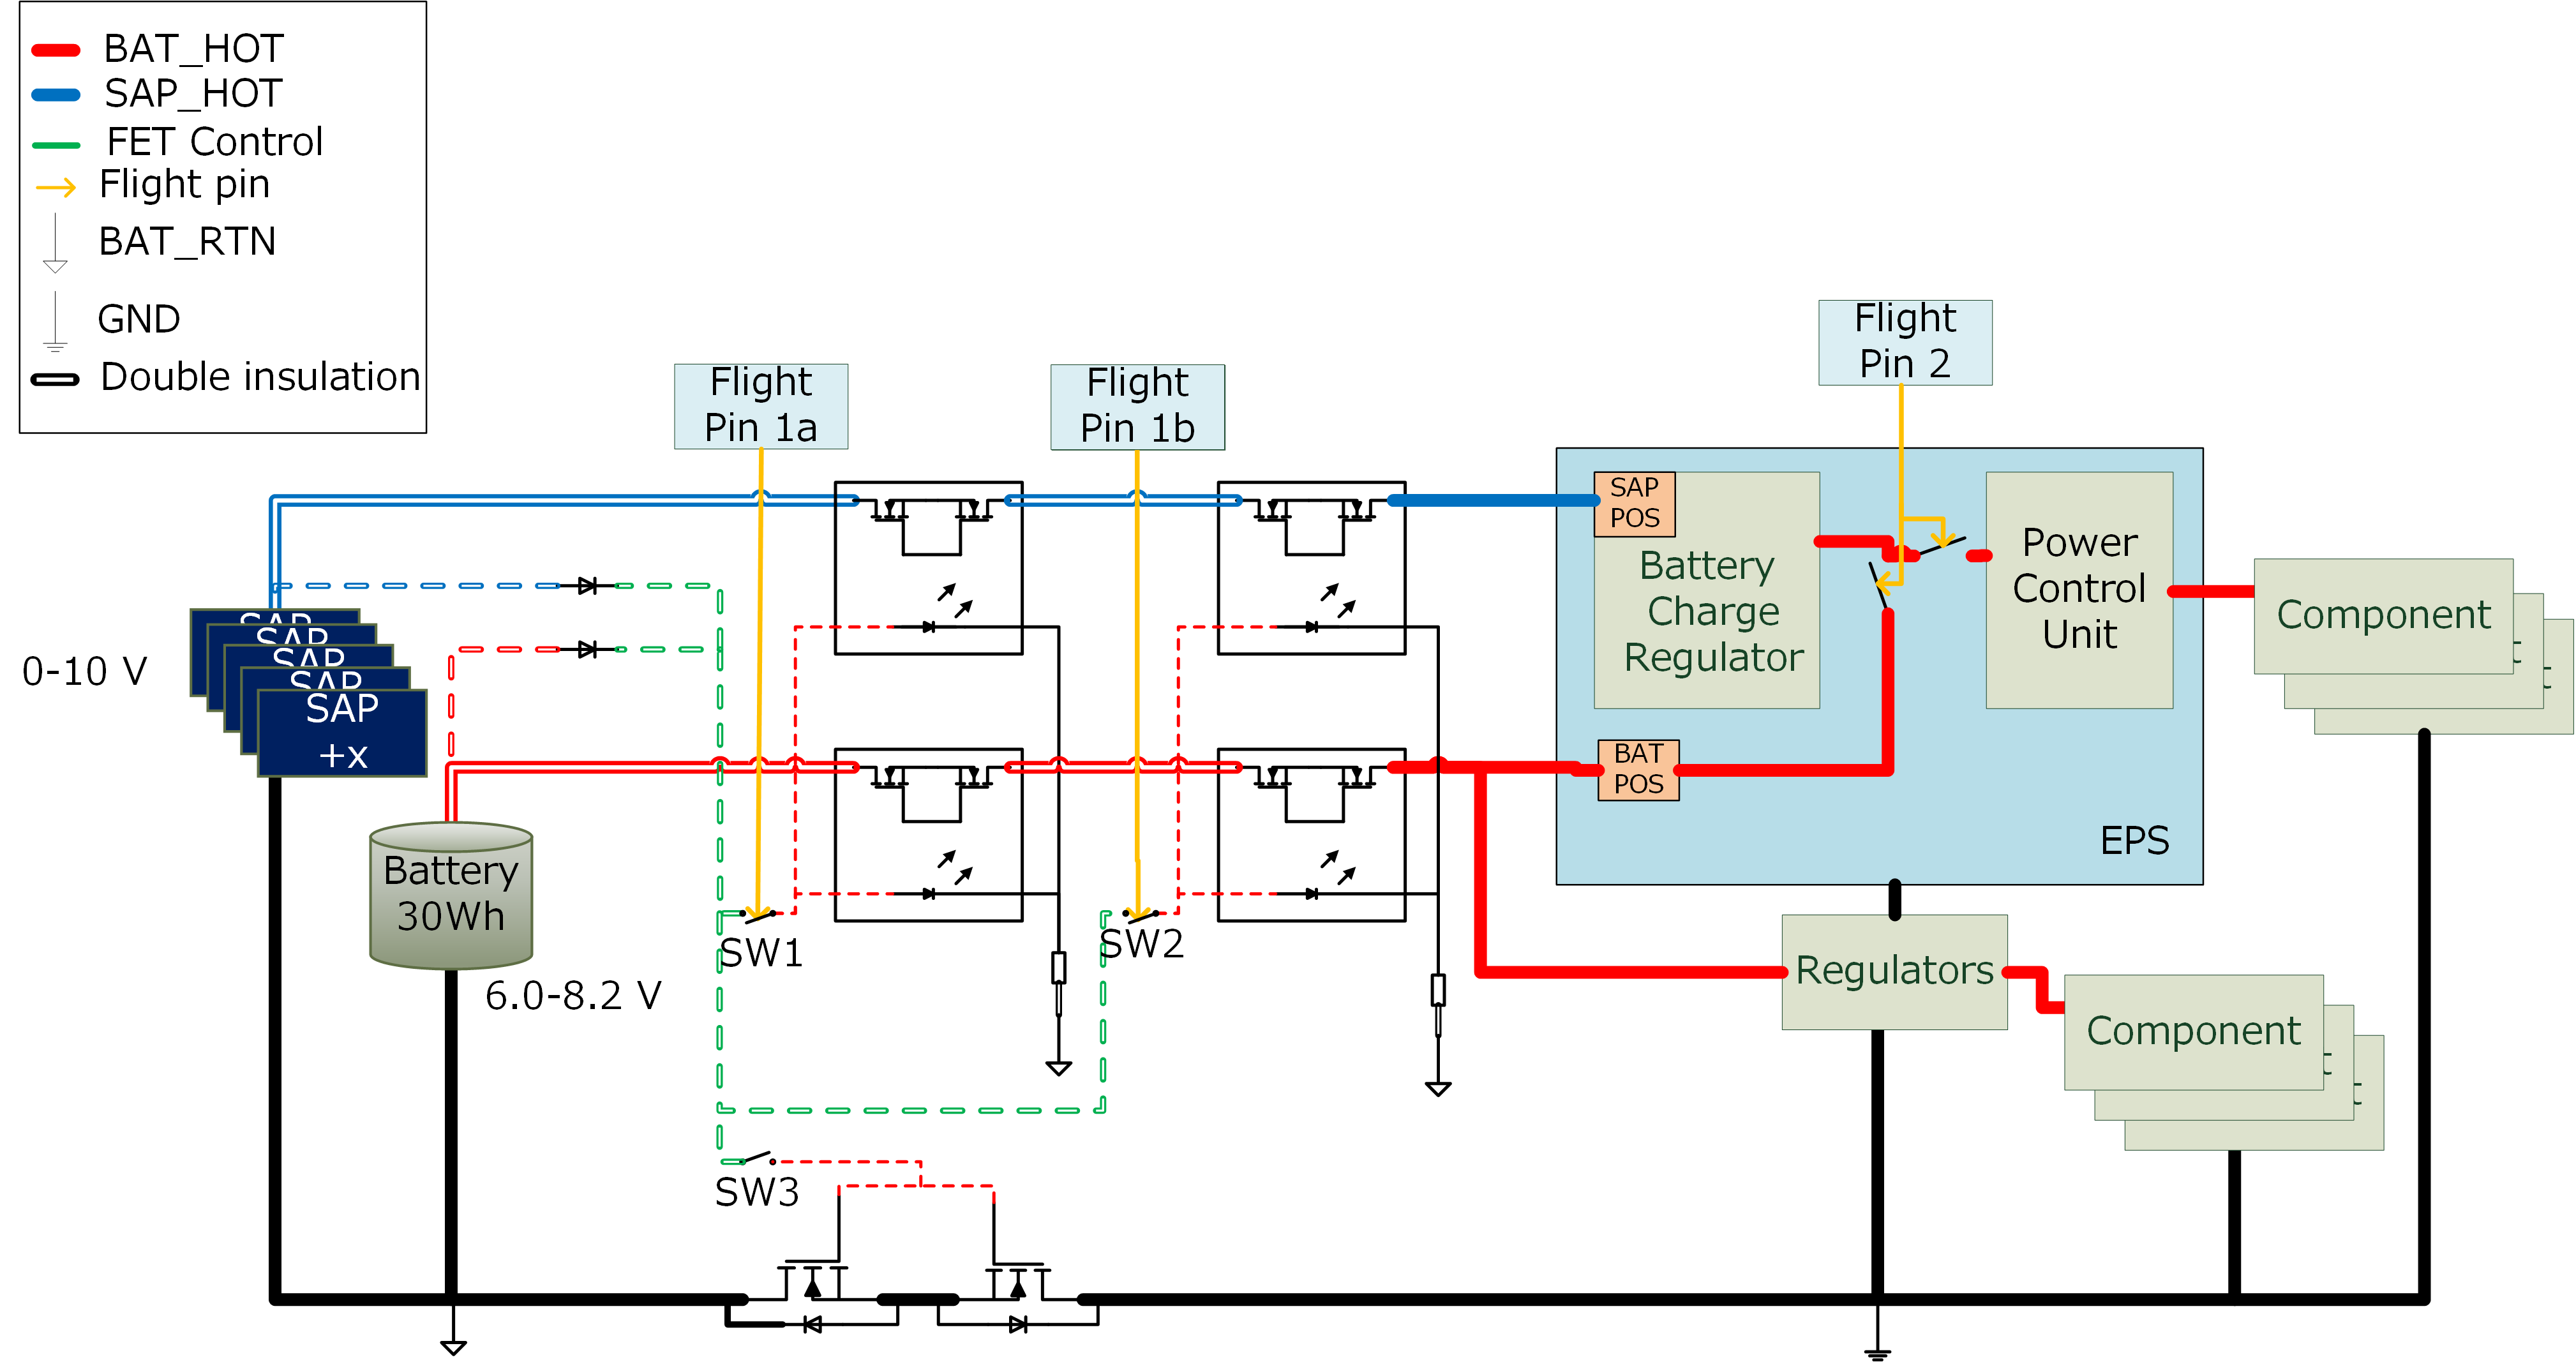
\includegraphics[width=0.9\linewidth]{./03/fig/inhibit_diagram_2.png}
		\caption{Inhibit Circuit Diagram}
		\label{fig3_1_inhibit_d}
	\end{center}
\end{figure}





